\section{Results}
We present our survey results and provide analyses of the data. We first discuss participants' responses to the various data-sharing scenarios, and how data type, data recipient, and device contributed to how threatening a situation was perceived. Next, we discuss participants' risk/benefit assessment of various new technologies relative to well-established technologies. We conclude the section with participants' self-reported concerns about the biggest risks in owning wearable devices.

\subsection{Concern Factors}
Many factors impact participants' concern levels for each scenario: the data recipient, the data type, and whether or not the scenario occurred on a wearable or a smartphone. We analyze each factor individually, as well as present a statistical model of participants' concerns as a function of all of factors, including demographic traits.

\subsubsection{Data Type}
Based on our data, we observed that the largest effect stemmed from the data type being shared in a scenario. We present various statistical models in section \ref{sec:regression} to support this conclusion. The 10 most and 10 least concerning data types can be seen in Table \ref{top10}. 

Regardless of the data recipient or the device, participants were most concerned about photos and videos, especially if they contained embarrassing content, nudity, or financial information. As seen in Table \ref{top10}, photos and videos accounted for 5 of the top 10 concerns. Information that could be used to impersonate someone (e.g., usernames/passwords for websites) or invade privacy (photos of someone at home) were also among the most concerning data types. 

Also regardless of the data recipient, the least concerning data types mostly consisted of information that could be observed through observations of public behavior, such as demographic information (e.g., age, gender, language spoken). It is possible that people rated these as unconcerning because they think many entities already track this data (e.g., shows watched, music listened to, exercise patterns).

\begin{table}[t]
\begin{center}
\small
\begin{tabular}{| r | l | r |}
\hline
Rank & Data &  VUR  \\
\hline
1 & a video of you unclothed & 95.97\% \\
2 & bank account information & 95.91\% \\
3 & social security number & 94.84\% \\
4 & video of you entering in your PIN & 92.67\% \\
5 & a photo of you unclothed & 92.59\% \\
6 & an incriminating/embarrassing photo of you & 91.39\% \\
7 & username and password for websites & 89.55\% \\
8 & credit card information & 88.98\% \\
9 & an incriminating/embarrassing video of you & 88.41\% \\
10 & a random (inward-facing) photo you at home & 87.50\% \\
 & \vdots & \\
64 & eye movement patterns (for eye tracking) & 40.51\% \\
65 & when and how much you exercise  & 38.66\% \\
66 & when you are happy or having fun  & 34.75\% \\
67 & which television shows you watch & 30.20\% \\
68 & when you are busy or interruptible  & 29.50\% \\
69 & music from your device  & 28.06\% \\
70 & your heart rate & 27.50\% \\
71 & your age & 24.29\% \\
72 & the language you speak & 15.86\% \\
73 & your gender & 15.00\% \\ 
\hline
\end{tabular}
\caption{The 10 most and least upsetting data types, across all recipients.}
\label{top10}
\end{center}
\end{table}

%A statistical analysis regarding the significance and confidence of <data> types with respect to all 72 was not performed due to the space constraints of the paper. We do consider all <data> categories in our statistical model, which provides an analysis of what factors had contributed to the perceived severity of a particular situation. 

\subsubsection{Data Recipient}
Across all scenarios, 42.3\% of participants stated that they would be ``very upset'' if their data was shared with only the app's servers, whereas the VURs for friends (69.5\%), work contacts (75.2\%), and the public (72.4\%) were much higher. A chi-square test indicated that these differences were statistically significant (Table \ref{recipient}). However, these effect sizes were small: the largest effect was between work contacts and an app's server ($\phi=0.11$); while the VUR for sharing with work contacts was significantly higher than sharing with friends, the effect size was negligible ($\phi=0.004$). 

We note that this chi-square test violates the assumption of independent observations, since participants responded to multiple scenarios. But based on the randomization of treatments and large sample size, we do not believe that this significantly impacted our results. Nonetheless, we repeated the analysis using only one randomly-selected data point per participant to find that the test was robust to this violation. Participants were significantly more concerned about having their data seen by humans ({\it vis-{\`a}-vis} app servers), though differences between specific human groups (between the public, friends, and work contacts) were not significant.

%Comment on differences between public/work, and end the subsection
%SE: this needs to be rewritten below.

We compared the 10 most concerning scenarios when sharing with an app servers versus with a humans. We observed that there was a substantial overlap between these groups, in that 6 of the most concerning scenarios were the same: \\[-.8cm]

\begin{packed_enum}
\item Bank account information
\item A video of you unclothed
\item Social security number
\item Video of you entering your PIN
\item An incriminating/embarrassing photo of you
\item A photo of you unclothed \\[-.8cm]
\end{packed_enum}

While the concerning data types do not appreciably change based on the data recipient---even the non-overlapping scenarios all dealt with confidential data (e.g., passcode, credit card information, etc.)---only the level of concern changed. For instance, the 10th most concerning scenario for the non-human audience had a VUR of 66.67\%, whereas the 10th most concerning scenario for a human audience has a VUR of 93.88\%. This suggests that concern for different data types does not appear to vary relative to other data types based on recipient, but instead the recipient determines the overall magnitude of the concern.\\

%\begin{table}[t]
%\begin{center}
%\begin{tabular}{|l|r|}
%\hline
%Recipients & VUR \\
%\hline
%App &  42.3\% \\
%Friends & 69.5\% \\
%Work & 75.2\% \\
%Public & 72.4\% \\ 
%\hline
%\end{tabular}
%\caption{generated for my presentation.}
%\label{nouse}
%\end{center}
%\end{table}


\begin{table}[t]
\begin{center}
\begin{tabular}{|l|r|r|r|r|}
\hline
Recipients	& $\chi^2$ & p-value 	& n & $\phi$ \\
\hline
Work-App	& 565.910 & <0.0001 & 5,083 & 0.111\\
Public-App	& 481.776 & <0.0001 & 5,1988& 0.093\\
Friends-App & 381.653 & <0.0001 & 5,096 & 0.075\\
Friends-Work & 20.39 & <0.0001 & 5,037 & 0.004\\
Friends-Public & 5.41 & <0.0200 & 5,142 & 0.001\\
Work-Public&  5.00 & <0.0253 & 5,129	& 0.001\\
\hline
\end{tabular}
\caption{Results of a chi-square test to examine VUR based on data recipient, across all data points.}
\label{recipient}
\end{center}
\end{table}

%\begin{table}[t]
%\begin{center}
%\begin{tabular}{|l|r|r|r|r|}
%\hline
%Recipients	& $\chi^2$ & p-value 	& n & $\phi$ \\
%\hline
%Work-App	& 42.49	& <0.0001	&	601	&	0.071\\
%Public-App &	48.52	& <0.0001	&		636	&	0.076\\
%Friends-App	& 32.07	& <0.0001	&		609	&	0.053\\
%Friends-Work & 	0.87 &	<0.3517	&	604	&	0.001\\
%Friends-Public	& 1.46 &	<0.2229	&	639	&	0.002\\
%Work-Public &	0.67 &	<0.7956	&		631	&	0.001\\
%\hline
%\end{tabular}
%\caption{Results of a chi-square test to examine VUR based on data recipient, across all data points.}
%\label{recipient}
%\end{center}
%\end{table}

%\begin{table}[t]
%\begin{center}
%\begin{tabular}{| c | c | c | c |}
%Recipients	& $\chi^2$ &	2-tail P &  Effect Size \\
%Work-App	& 564.318 & <0.0001 & 0.111\\
%Public-App	& 479.980 & <0.0001 &  0.092\\
%Friends-App & 380.000 & <0.0001 & 0.075\\
%Friends-Work & 20.365 & <0.0001 &  0.004\\
%Friends-Public & 5.349 & 0.0207 &  0.001\\
%Work-Public&  5.054 & 0.0246 &  0.001\\
%\end{tabular}
%\caption{Chi-Squared test results of the effects of various recipients contributing to VUR.}
%\label{recipient}
%\end{center}
%\end{table}				

%\begin{table}[t]
%\begin{center}
%\begin{tabular}{| l | c |}
%<data> & VUR  \\
%social security number & 98.04\% \\ CC
%a video of you unclothed & 97.44\% \\ CC
%bank account information & 97.10\% \\ CC
%recordings of your work conversations & 96.97\% \\ 
%an incriminating/embarrassing photo of you & 96.36\% \\ CC
%a photo of you unclothed & 96.30\% \\ CC
%credit card information & 95.92\% \\ 
%username and password for websites & 95.41\% \\ 
%a video of you entering in your PIN & 93.91\% \\ CC
%recordings of your phone conversations & 93.88\% \\ 
%\end{tabular}
%\caption{A table of the top 10 upsetting <data> types, with respect to <recipient> types friends, work, and public.}
%\label{sharedtop10}
%\end{center}
%\end{table}
%
%\begin{table}[t]
%\begin{center}
%\begin{tabular}{| l | c |}
%%starting from #63
%<data> &  VUR  \\
%bank account information & 90.91\% \\ CC
%a video of you unclothed & 90.62\% \\ CC
%social security number  & 88.68\% \\ CC
%video of you entering your PIN & 88.57\% \\ CC
%an incriminating/embarrassing photo of you & 78.05\% \\ CC
%a photo of you unclothed & 77.78\% \\ CC
%a video of you entering a passcode to a door & 75.00\% \\ 
%when and how much you have sex & 73.08\% \\ 
%an incriminating/embarrassing video of you & 71.88\% \\ 
%a random (inward-facing) photo of you at home & 66.67\% \\
%\end{tabular}
%\caption{A table of the top 10 upsetting <data> types, respect to <recipient> app's server only (didn't share it with anyone else).}
%\label{notsharedtop10}
%\end{center}
%\end{table}
%
%\begin{table}[t]
%\begin{center}
%\begin{tabular}{| l | c |}
%%starting from #63
%<data> &  VUR  \\
%your name & 47.25\% \\
%when and how much you exercise & 46.07\% \\
%when you were happy or having fun & 38.10\% \\
%what television shows you watch & 35.96\% \\
%when you are busy or interruptible & 34.34\% \\
%your heart rate & 32.28\% \\
%music from your device & 31.87\% \\
%your age & 29.67\% \\
%the language you speak & 20.95\% \\
%your gender & 16.81\% \\
%\end{tabular}
%\caption{A table of the bottom 10 upsetting <data> types, with respect to <recipient> types friends, work, and public.}
%\label{sharedbottom10}
%\end{center}
%\end{table}
%
%
%\begin{table}[t]
%\begin{center}
%\begin{tabular}{| l | c |}
%%starting from #63
%<data> &  VUR  \\
%when and how much you exercise & 16.67\% \\
%how much you use your phone & 15.79\% \\
%your age & 14.29\% \\
%how much you like the people you interact with & 13.79\% \\
%when, what, and how much you ate & 12.50\% \\
%which television shows you watch & 11.43\% \\
%your gender & 9.52\% \\
%your heart rate & 9.09\% \\
%eye movement patterns (for eye tracking) & 6.98\% \\
%the language you speak & 2.50\% \\
%\end{tabular}
%\caption{A table of the bottom 10 upsetting <data> types, respect to <recipient> app's server only (didn't share it with anyone else).}
%\label{notsharedbottom10}
%\end{center}
%\end{table}
%
%Commonly, bank info, SSN, PIN, embarrassing photo, naked photo, naked video were considered to be highly sensitive. When people perceived that the data would be shared with the app only, the other top five concerns included the passcode to a door, how frequently one has sex, embarrassing videos, and photos at home. When people perceived that the data would be shared with a human audience, their other top concerns were work conversations, credit card information, username and password combinations for websites, and phone conversations. When data is perceived to be shared by an app, people are more concerned with issues of being spied on or tracked, whereas when data is perceived to be shared with an individual, people are concerned more with theft or reputation. 
%
%On the other hand, exercise details, age, tv shows, gender, heart rate, and language were commonly considered to be lease concerning. When people perceived that the data would be shared with the app only, the other indifferent data included phone use, how much one liked the people around, when and what you ate, and eye patterns. When people perceived that the data would be shared with a human audience, the least concerning data included one's name, if one was having fun, music on the device, and if one was busy or interruptible. When sharing with an application, information otherwise considered personal such as phone use, opinions of people, food eaten, or eye patterns were okay to share, since these seem like useful information to improve one's device experience. However, people are not likely to share the same with people, but are more comfortable with sharing data about topics which would come up in causal conversation.

\subsubsection{Device}
Participants had unique VURs for scenarios only differing in device. Our participants had a 58.79\% VUR when asked about wearables and 46.64\% VUR when asked about smartphones.The VURs for both devices for all 5 questions are in table ~\ref{deviceVUR}. However, the effect the device has on the VUR is not considered to be statistically significant (see Table ~\ref{betweendevice}). Additionally, there is no statistically significant difference between how people reacted in a given situation; although, participants were statistically significantly upset in Q2. The aforementioned results are only with respect to between subjects analysis, where answers are from participants who received either only the wearables or smartphone version of the 5 questions. Too few instances of participants answering both versions of questions occured (34 in total for all 5 questions) to perform a sound within-subjects analysis. 

\begin{table}[t]
\begin{center}
\begin{tabular}{| c | r | r |}
\hline
 Question &  Wearable VUR & Smartphone VUR \\
 \hline
 All & 58.79\% & 46.64\%\\
Q1 & 14.81\%  &  6.13\%\\
Q2 & 44.11\%  &  19.85\%\\
Q3 & 87.09\%  &  58.44\%\\
Q4 & 52.77\%  & 55.74\%\\
Q5 & 86.49\%  &  91.82\%\\ 
\hline
\end{tabular}
\caption{VURs for the questions described in Section \ref{sec:smartphones}, contrasting smartphones with the Cubetastic3000.}
\label{deviceVUR}
\end{center}
\end{table}

\begin{table}%[h]
\begin{center}
\begin{tabular}{|c|r|r|r|r|}
%Question & Chi^2 &	2-tail P &	Sig?	 & n	& effect size\\
%All	2.814	0.1395	No		3589		0.001\\
%Q1	2.500	0.1139	No		714		0.004\\
%Q2	17.333	<0.0001	Yes		708		0.024\\
%Q3	0.020	0.8886	No		699		0.000\\
%Q4	1.426	0.2324	No		731		0.002\\
%Q5	1.611		0.2043	No		710		0.002\\
\hline
Question & $\chi^2$ & p-value & n & $\phi$ \\
\hline
All & 2.202 & <0.1378 & 3,588 & 0.001\\
Q1 & 2.500 & <0.1139 & 714 & 0.004\\
Q2 & 17.333 & <0.0001 & 708 &  0.024\\
Q3 & 0.020 & <0.8886 & 699 &  0.000\\
Q4 & 1.413 & <0.2345 & 730& 0.002\\
Q5 & 1.604 & <0.2054 & 709 & 0.002\\
\hline
\end{tabular}
\caption{Chi-square test results comparing participants' VURs between the smartphone and Cubetastic3000 questions.}
\label{betweendevice}
\end{center}
\end{table}
						
%\begin{table}%[h]
%\begin{center}
%\begin{tabular}{| c | c | c | c |}
%Question & $\chi^2$ &	2-tail P & Effect Size \\
%All & 0.444  & 0.505 & 0.006\\
%Q1 & 0 & 1 & 0 \\
%Q2 & 0 & 1 & 0\\
%Q3 & 0 & 1 & 0\\
%Q4 & 0 & 1 & 0\\
%Q5 & 0 & 1 & 0\\
%\end{tabular}
%\caption{Results of the effects of <device> type contributing to VUR. Values are McNeamar's test results for within-subjects comparisons for participants who received both questions.}
%\label{withindevice}
%\end{center}
%\end{table}

%For the between-subjects comparison (i.e., participants who received one question, but not the other), you can do either a chi-square test or Fisher's exact test. Both use a 2 x 2 contingency matrix (i.e., rows are outcomes---upset or not---and columns are conditions---wearable or smartphone). The way to choose between the two tests is based on sample size, generally you use chi-square when there are more than 10-20 samples per cell in the table, but using either is just as valid. For the within-subjects comparisons (i.e., participants received both questions), you would do McNemar's test; which is the within-subjects version of the chi-square test. 

\subsubsection{Demographic Factors}

Participants' responses were correlated with demographic factors. We observed that the biggest predictor of participants' decisions to rate a scenario as very upsetting was their self-reported level of general privacy concerns, as determined by the IUIPC scale~\cite{malhotra2004internet}: a Spearman correlation yielded a statistically significant effect between average IUIPC scores with the VUR ($\rho=0.446$, $p<0.0005$). Similarly, we observed that age was a significant predictor of VUR ($\rho=0.121$, $p<0.0005$). We suspect that the effect of age is due to the significant correlation between age and IUIPC scores ($\rho=0.188$, $p<0.0005$); others have observed that older individuals tend to be more protective of their privacy~\cite{varian2005demographics}.

While we initially observed an effect on VURs based on whether or not participants claimed to already own wearable devices (57.0\% vs. 60.8\%, respectively; Mann-Whitney $U=202,896$, $p<0.032$), this difference did not remain significant upon correcting for multiple testing (Bonferroni corrected $\alpha=0.01$), nor did the effect of gender. Finally, we observed no correlation between education level and VUR.

\subsubsection{Regression Models} 
\label{sec:regression}
In order to examine the relative effect of each factor on participants' VURs, we constructed several statistical models to predict whether a participant would be ``very upset'' with a given scenario based on the data type, device, data recipient, and their demographic factors (i.e., age, education, gender, and privacy attitudes). We performed binary logistic regressions using generalized estimating equations, which account for our repeated measures experimental design (i.e., each participant contributed multiple data points).

\begin{table}
\centering
\begin{tabular}{|l| r| r| r|}
\hline
Parameters & $\chi^2$ & $df$ & QIC\\
\hline
\hline
(Intercept) & 255.0 & 1 & 18,477.5\\
\hline
(Intercept) & 78.4 & 1 & 18,122.9\\
Device & 400.3 & 1 & \\
\hline
(Intercept) & 289.1 & 1 & 17,667.5\\
IUIPC (covariate) & 368.5 & 1 & \\
\hline
(Intercept) & 297.8 & 1 &17,383.6\\
Data Recipient & 913.4 & 4 & \\
\hline
(Intercept) & 374.6 & 1 & 14,794.5\\
Data Type & 1,866.5 & 77 & \\
\hline
(Intercept) & 303. & 1 & 13,942.9\\
Device & 11.1 & 1 &  \\
Data Recipient & 624.6 & 3 & \\
Data Type & 1,961.2 & 76 &  \\
\hline
(Intercept) & 28.4 & 1 & 12,752.8 \\
Device  & 8.8 & 1 &  \\
Data Recipient & 577.8 & 3 & \\
Data Type & 1,752.1 & 76 & \\
IUIPC (covariate) & 378.7 & 1 & \\
\hline
\end{tabular}
\caption{Goodness-of-fit metrics for various binary logistic models of our data using general estimating equations to account for repeated measures. The columns represent the Wald test statistic for each parameter and the overall Quasi-Akaike Information Criterion (QIC) for each model.}
\label{regression}
\end{table}

We created several models using our three dependent variables as factors: device (smartphone vs. wearable), data recipient, and data type. We also used our collected demographic factors as covariates: age, gender, education, wearable device ownership (yes/no), and mean IUIPC score. For each model, we performed Wald's test to examine the model effects attributable to each of these eight parameters and observed that the only covariate that had an observable effect on our models was participants' IUIPC scores. Thus, we opted to remove the other covariates from our analysis.

Table \ref{regression} shows the various models that we examined and the Quasi-Akaike Information Criterion (QIC), which is a goodness-of-fit metric for model selection (lower relative values indicate better fit). As can be seen, while the remaining four predictors all contributed to the predictive power of our model, the data type was the strongest predictor. Conversely, despite being significant, the device was the weakest predictor (i.e., whether participants were answering questions about a smartphone or a wearable device).


\subsection{Risk and Benefit Rankings} 
\begin{figure}[t]
	\centering
	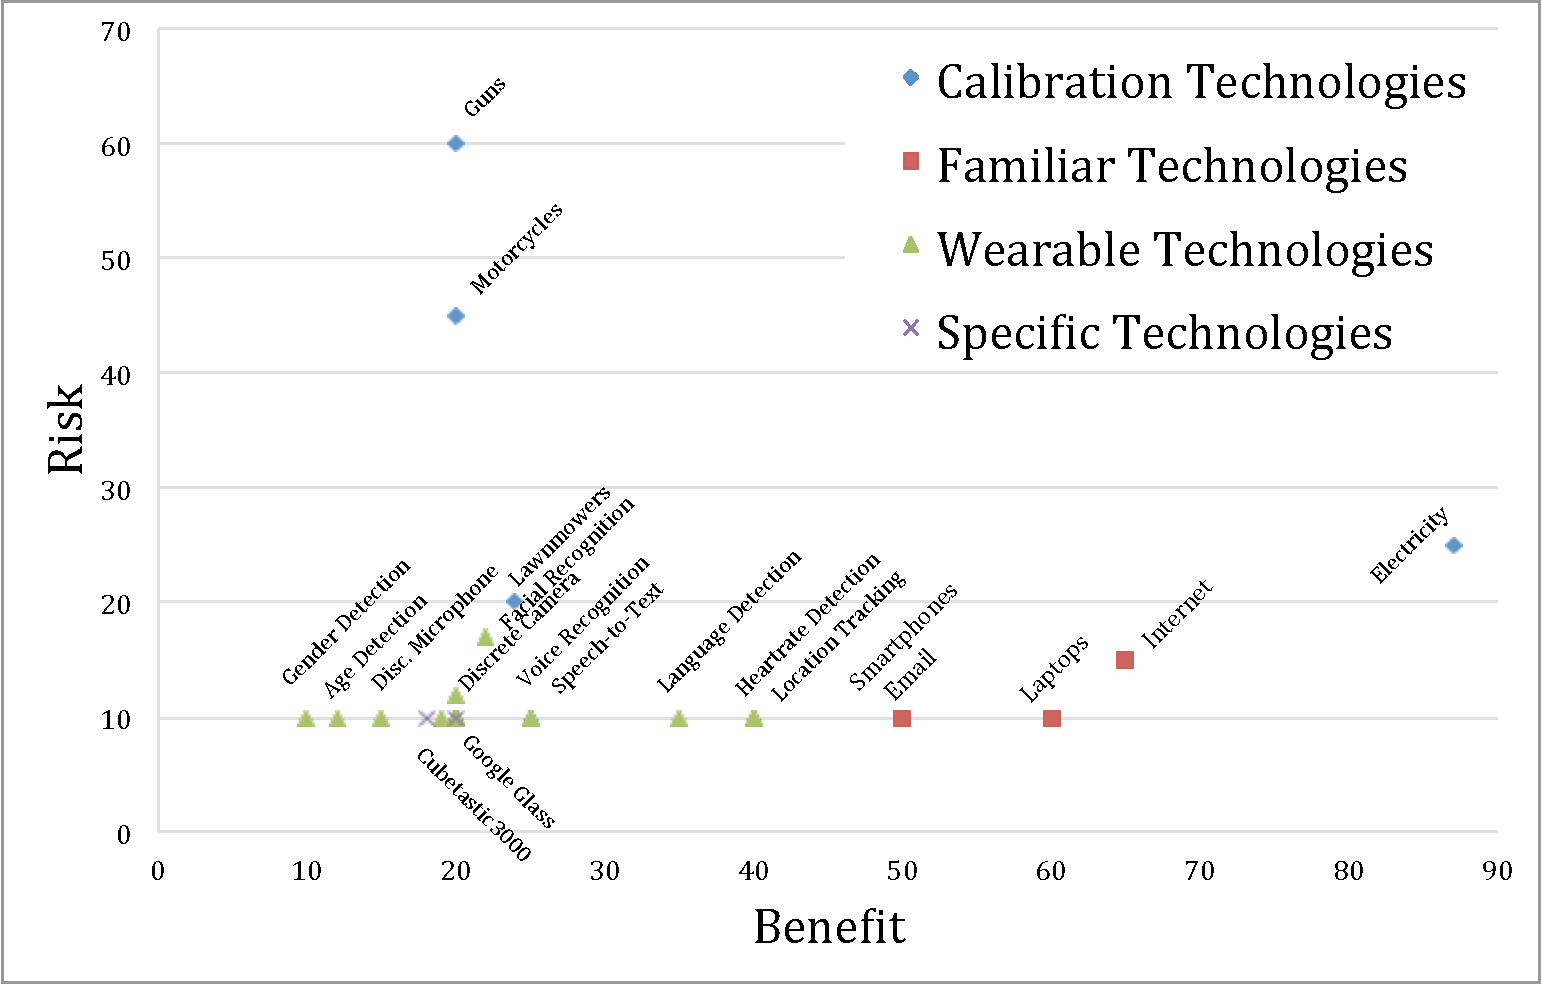
\includegraphics[width=0.47\textwidth]{images/riskbenefit.pdf}
	\caption{Participants' median risk-benefit ratings of technologies examined by Fischhoff \etal\cite{Fischhoff}, which we used for calibration, alongside familiar technologies (e.g., laptops, the Internet, etc.), wearable technologies, as well as two specific wearable devices (Google Glass and the Cubetastic3000).}
	\label{fig:techplot}
\end{figure}

We asked participants to rate new capabilities related to wearable technologies (e.g., facial recognition) in terms of their risks and benefits. We also asked them to do this for technologies with which they were likely to be more familiar (e.g., smartphones and laptops) in addition to two examples of specific wearable devices, Google Glass and the fictitious Cubetastic3000. To calibrate our results, we also asked about four well-established technologies studied by Fischhoff \etal\cite{Fischhoff}. We found that participants generally rated familiar technologies and those related to wearables as being low-risk. Figure~\ref{fig:techplot} depicts participants' median ratings. We found that the calibration technologies were all rated as the most risky. At the same time, with the exception of electricity, the calibration technologies were seen as lower benefit than the others.

As a group, participants rated the familiar technologies as the most beneficial. We believe this is the result of exposure people have to these technologies---most people use these technologies daily. Of the wearable technologies, the most risky were ones perceived to be privacy-invasive; the most risky technologies were facial recognition, the Internet, and discrete cameras, whereas the remainder of the technologies were seen as having minimal---albeit equivalent---risk levels (i.e., a median of ``10''). People are becoming increasingly aware of such privacy risks and are comparing these privacy invasion to real physical risks--for instance, the capacity for facial detection on a wearable device is perceived to be almost as risky as interacting with a lawnmower.

These perceptions of the most risky or beneficial technologies may not be reflective of actual risks or benefits. However, they do reflect the general public's exposure to these technologies and show that people perceive specific risks and benefits. We suspect that the similarity in assessments between the various wearable technologies are because most people are not consciously aware of the possibilities of these technologies or how they could be used. We suspect that performing this experiment longitudinally may yield more interesting results, as these technologies become more and more pervasive (and therefore more familiar to participants).

\subsection{Self-Reported Concerns for Wearables}
We also wanted to capture the participants' general reactions to wearable devices as a whole. To do this, we asked the participants the following open-ended question:

\textit{What do you think are the most likely risks associated with wearable devices?}\\[-.5cm]

This question was asked along with demographics questions (but before any IUIPC questions to avoid biasing). The participants were presented with a blank box to write in, with no character limit to their open-ended responses. \\

Without a doubt, the most common self-reported concern of wearables for the average user is the \textit{possible loss of privacy} (see Table \ref{openresponses}). Other significant secondary concerns included being unaware of what the device is collecting, doing, or which information it is using (Being Unaware), long-term health effects caused from wearing the device such as cancer from emf waves (Health), safety hazards from wearing the device such distractions causing car accidents (Safety), resulting changes in social behaviors, such as dependencies on devices or spending less time with loved ones (Social Impact), the high financial cost of buying, replacing, or caring for the device (Financial), and information compromise (Security).

\begin{table}[t]
\begin{center}
\begin{tabular}{|l|r|r|}
\hline
Concern &  Responses &  Frequency   \\
\hline
Privacy & 452 & 25.32\% \\
Being Unaware & 275 & 15.40\% \\
%Unaware Use & 167 & (9.36\%)\\
%Unaware Collection & 64 & (3.59\%)\\
%Unaware Access & 44 & (2.46\%)\\
Health Risk & 191 & 10.70\%\\
Safety & 185 & 10.42\%\\
Social Impact &	157 & 8.80\%\\
Financial Cost & 151 & 8.46\%\\
Security &	144 & 8.07\%\\
Accidental Sharing &	69 & 3.87\%\\
Miscellaneous &	57 & 3.19\%\\
None	& 51 & 2.86\%\\
Social Stigma &	39 & 2.18\%\\
False Information & 33 & 1.85\%\\
Don't know & 31 & 1.74\%\\
Aesthetics 	& 19 & 1.06\%\\
Don't care 	& 11 & 0.62\%\\
\hline
\end{tabular}
\caption{A table listing the self-reported most common risks associated with owning a wearable device.}
\label{openresponses}
\end{center}
\end{table}